\documentclass[a4paper]{article}

\usepackage[utf8]{inputenc}
\usepackage[ngerman]{babel}
\usepackage[autostyle=true,german=quotes]{csquotes}
\usepackage{amsmath}
\usepackage{amssymb}
\usepackage{graphicx}

\author{Paul Brinkmeier}
\title{Cheatsheet für Einführung in Rechnernetze}

\begin{document}
	\maketitle
	\newpage
	\tableofcontents
	\newpage

	\section{Grundlegende Grundlagen}

	\paragraph{Rechnernetz}

	Ein Rechnernetz besteht aus Komponenten und Übertragungsmedien, die diese Komponenten miteinander verbinden.
	Übertragungsmedien realisieren die sogenannten Kommunikationslinks (Übertragungsstrecken) zwischen Komponenten.

	Komponenten sind beispielsweise Computer, Smartphones, Kühlschränke, Router.

	Medien sind beispielsweise Koaxialkabel, Kupferkabel, Glasfaser, Funk.

	\paragraph{Endsystem}

	Endsysteme (Hosts) führen verteilte Anwendungen aus.
	Diese benötigen ein Rechnernetz zur Kommunikation zwischen Anwendungsinstanzen.
	Beispiele für verteilte Anwendungen und Endsysteme: WhatsApp auf Smartphone, E-Mail auf Server, etc.

	\paragraph{Zwischensystem}

	Zwischensysteme leiten Daten im Netz weiter und führen i.d.R. keine verteilten Anwendungen aus.
	Beispiele für Zwischensysteme: Router, Switch.

	\paragraph{(Kommunikations-)Protokoll}

	Protokolle definieren Regeln und Formate für die Kommunikation zwischen zwei oder mehreren Computern sowie die beim Senden und Empfangen von Daten bzw. bei Ereignissen auszuführenden Aktionen.

	\paragraph{(Daten-)Pakete}

	Die von Anwendungen zu sendenden Daten können in kleinere Teile gegliedert werden.
	Diese werden als (Daten-)Pakete bezeichnet.
	Pakete sind aufgebaut aus Metadaten und Nutzdaten.
	Metadaten sind nur für die Abwicklung des Protokolls erforderlich; Nutzdaten sind die eigentlichen für die Anwendung wichtigen Daten.
	I.d.R. werden Pakete in Rechnernetzen unabhängig voneinander bearbeitet.

	\paragraph{Datenrate (Übertragungsrate)}

	Die Datenrate bezeichnet die Geschwindigkeit, mit der Daten zwischen zwei Komponenten übertragen wird.
	Sie wird in bit/s gemessen.
	Größenordnungen: K, M, G, T, etc. \emph{nicht} Ki, Mi, Gi, Ti!

	\subsection{Netzkern und Netzrand}

	\paragraph{Netzkern}

	Der Netzkern besteht aus den Netzen untereinander verbunderer Internet Service Provider (ISPs).
	Er beschäftigt sich vor allem mit der Weiterleitung von Paketen.
	Der Netzkern ist sozusagen das \enquote{Betriebssystem} des Internets.

	\paragraph{Netzrand}

	Der Netzrand besteht aus den Netzen von Endandwendern, bspw. Heimnetze, Firmennetze und Datenzentren.
	Er beherbergt die \enquote{Anwendungen} des Internets.

	\subsection{\enquote{Provider} im Internet}

	\paragraph{Internet-Service-Provider (ISP)}

	ISPs binden Konsumenten an das Internet an.
	Dazu gehören oft tausende Kunden und auch Unternehmen.
	Bspw. Unitymedia, Telekom, 1\&1.

	Verschiedene Größenordnungen: Tier-1-ISP, Regionaler ISP, Zugangs-ISP.

	\subparagraph{Warum hierarchisch?}

	Vernetzung aller $n$ Zugangs-ISPs Verbindungen $\in O(n^2)$ $\leadsto$ skaliert nicht.

	\paragraph{Internet-Exchange-Point (IXP)}

	IXPs sorgen für Datenaustausch zwischen größeren ISPs.
	Es gibt weltweit ca. 400 IXPs.

	\paragraph{Content-Provider}

	Content-Provider erzeugen und stellen Inhalte bereit.
	Sie wollen diese so nah wie möglich an den Netzrand ($\leadsto$ zu den Kunden) bringen.
	Bspw. Google, Netflix, Amazon.

	\subsection{Modellierung}

	\paragraph{Modell}

	Ein Modell ist ein vereinfachtes Abbild der Wirklichkeit.
	Man setzt Modelle ein, um die wesentlichen Aspekte eines Systems darzustellen.
	Die innere Struktur des Systems wird abstrahiert; man modelliert die Interaktion mit dem System (Black-Box).

	\subsubsection{Grundmodell der Kommunikation}

	\begin{itemize}
		\item Sender und Empfänger (je einer oder mehrere).
		\item Abstraktes Medium.
	\end{itemize}

	\paragraph{Abstraktes Medium}
	
	Das Medium verbindet Sender und Empfänger über eine räumliche Distanz.
	Es stellt damit einen (Kommunikations-)Dienst zur Verfügung.
	Den Übergang von Sender/Empfänger zum Medium nennt man Schnittstelle.

	Ein abstraktes Medium trifft keinerlei Aussage über seine konkrete (physische) Umsetzung.

	\paragraph{Dienstesicht}

	Betrachtung eines Rechnernetzes als Black-Box.
	Das RN erbringt einen Dienst für seine Nutzer.

	Das RN entspricht hier dem abstrakten Medium.

	\paragraph{Dienst}

	Ein Dienst bündelt zusammengehörige Funktionen und stellt diese einem Nutzer (Dienstnehmer) zur Verfügung.
	Einzelen Teile eines Dienstes können unabhängig voneinander in Anspruch genommen werden.

	Ein \emph{Dienstzugangspunkt} (Service Access Point, SAP) stellt die Schnittstelle zu einem Dienst dar.

	\emph{Dienstnehmer} nehmen eine Dienst in Anspruch.

	\emph{Dienstgeber} (Diensterbringer) stellen einen Dienst zur Verfügung.

	\emph{Dienstprimitive} beschreiben die Interaktionen zwischen Dienstnehmer und Dienstgeber.

	Die \emph{Beschreibung eines Dienstes} reflektiert das Verhalten an den Dienstzugangspunkten zum Dienstgeber.

	\begin{figure}
		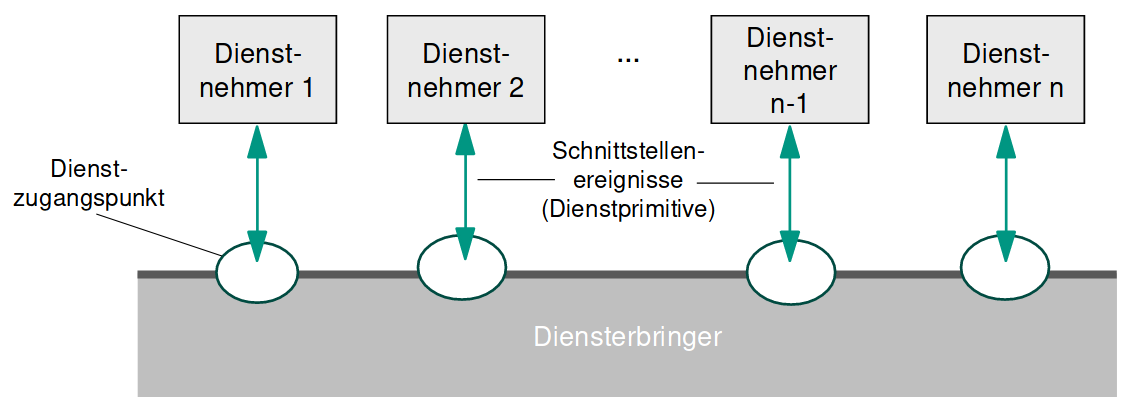
\includegraphics[width=\textwidth]{images/02-services.png}
		\caption{Dienstesicht}
	\end{figure}

	\paragraph{Dienstprimitive}

	\begin{itemize}
		\item \emph{Request} (req) --- Dienstnehmer 1 (DN1) beauftragt Dienstgeber.
		\item \emph{Indication} (ind) --- Dienstgeber benachrichtigt Dienstnehmer 2 (DN2) über Auftrag.
		\item \emph{Response} (res) --- DN2 beantwortet Auftrag.
		\item \emph{Confirmation} (cnd) --- Dienstgeber benachrichtigt DN1 über Abschluss.
	\end{itemize}

	\begin{figure}
		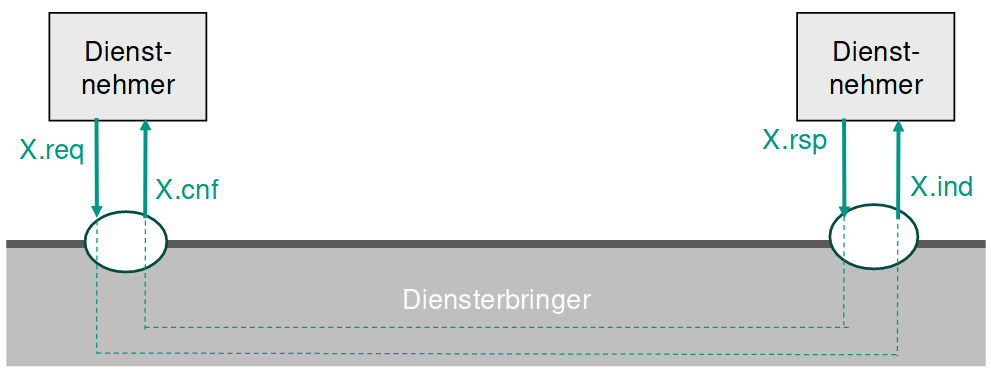
\includegraphics[width=\textwidth]{images/02-primitives.png}
		\caption{Dienstprimitive}
	\end{figure}

	\paragraph{Formen von Diensten}

	\begin{itemize}
		\item Unbestätigter Dienst --- Request (DN1), Indication (DN2).
		\item Bestätigter Dienst --- Request (DN1), Indication (DN2), Response (DN2), Confirmation (DN1).
	\end{itemize}

	\begin{figure}
		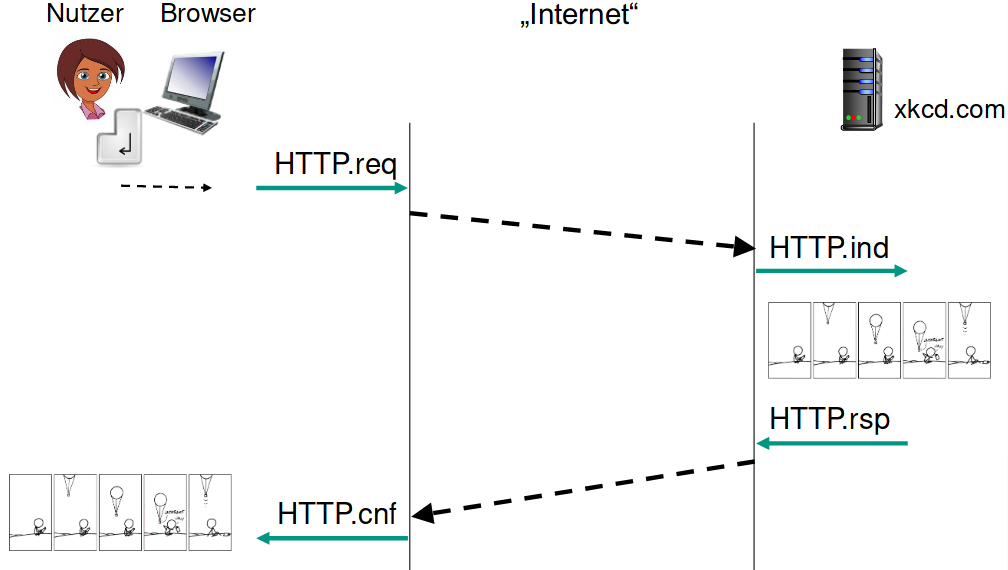
\includegraphics[width=\textwidth]{images/02-http-example.png}
		\caption{Beispiel für einen bestätigten Dienst: HTTP}
	\end{figure}

	\subsection{Zuverlässiger Dienst}

	\paragraph{Zuverlässiger Dienst}

	Bei einem zuverlässigen Dienst gilt am Dienstzugangspunkt des Empfängers folgendes:

	\begin{itemize}
		\item Alle empfangenen Daten sind korrekt.
		\item Alle vom Sender zu empfangenden Daten werden vollständig und in der richtigen Reiehnfolge empfangen.
		\item Es werden keine Duplikate empfangen.
		\item Es werden keine Phantom-Daten empfangen.
	\end{itemize}

	\section{Physische Schicht}

	\section{Sicherungsschicht}

	\section{Vermittlungsschicht}

	\section{Transportschicht}

	\section{Anwendungsschicht}

	\section{Netzssicherheit}

	\section{Klausuraufgaben}
\end{document}
